\chapter{Linear Cross Entropy}
\label{ch:lxe}
\epigraph{Check the circuit}{Spock to helmsman;
  \citefield{butlerCage1988}{booktitle}
--- \citefield{butlerCage1988}{number}}

PTIM: \cite{langEntanglementTransitionProjective2020}

Fisher/Altman PRL, hier wird die LXE definiert: \cite{liCrossEntropyBenchmark2023}

Nicolai: \enquote{Das ist eines der Paper, die Fisher zitiert, wo die LXE eingeführt wurde.} \cite{baoSymmetryEnrichedPhases2021}

arXiv:2306.00058, LXE fürs PTIM, preprint \cite{tikhanovskayaUniversalityCrossEntropy2023}

MIPT allgemein, hier leider eher weniger ahnung warum ich das in dieses Kapitel rein
gemacht hab zum zitieren. \cite{baoTheoryPhaseTransition2020}

Sampling stuff aus appendix von \cite{roserDecodingProjectiveTransverse2023}

As already touched upon in \cref{sec:sampling}, entanglement transitions elude
any measurement we could perform in an experiment. In this chapter we will
investigate a measure proposed by \citeauthor{liCrossEntropyBenchmark2023} and
specifically apply it to the projective transverse-field Ising model (PTIM). We
will first go over the definition and some properties before moving on to the
computation of the linear cross entropy and the numerical implementation. We
further discuss some interesting features
\section{Linear Cross Entropy \& Stabilizer}
In this section we provide a definition for the linear cross entropy (LXE)
$\chi$ and a detailed derivation for its computation in Clifford circuits.

Hier Definition und die ganze algebra/mathematik. dann den part zu LXE in
stabilizer (mit dieser projection und so)

Auch verschiedene Trackings?

\subsection{Definition and properties}
We first introduce the linear cross entropy (also abbreviated as LXE) in the
context of general random quantum circuits. We then provide a concrete
description and expression of the LXE for our system, the projective
transverse-field Ising model.

Consider a hybrid circuit with some cicruit layout $C$, consisting of unitary
and measurement gates. The measurement gates within the circuit yield results
$m_i$, which are collected in the sequence $\mathbf{m} = \{m_1, m_2, \ldots,
m_N\}$, where $N$ is the number of measurement gates. We call this sequence of
measurement outcomes the \emph{measurement record}. For some initial state
$\rho$ of our hybrid circuit, we can compute the \emph{unnormalized} output
state as
\begin{align}\label{eq:rho-m}
  \rho_\mathbf{m} \equiv C_\mathbf{m} \rho C^\dagger_\mathbf{m}
.\end{align}
Here, $C_\mathbf{m}$ is the time-ordered product of all gates in the circuit,
unitary and measurement, and can be written as
\begin{align}
  C_\mathbf{m} = 
.\end{align}
The action of $C_\mathbf{m}$ on the initial state
$\rho$ is the mathematical object representing one possible trajectory with
measurement outcomes $\mathbf{m}$. Leaving the state unnormalized after 
projection operations is a deliberate choice; it allows us to define the
probability of a certian measurement record.

\begin{defn}[Probability of a trajectory]\label{defn:prob-traj}
  Given a random circuit $C$ and an initial state $\rho$ with corresponding
  measurement record $\mathbf{m}$, the probability of $\mathbf{m}$ is denoted
  by
  \begin{align}
    P\left( \mathbf{m} \mid C, \rho \right) \equiv \Tr[\rho_\mathbf{m}] =
    \Tr[C_\mathbf{m} \rho C^\dagger_\mathbf{m}]
  .\end{align}
\end{defn}

Although we do not want to delve too deep into probability theory at this point,
let us nonetheless first convince ourselves that \cref{defn:prob-traj} really does
define a proper probability measure. To this end, consider the simplest example of
a circuit with initial state $\rho = \dyad{+}$ and a single measurement in the
Pauli-$Z$ basis. By \cref{eq:rho-m} our unnormalized output state reads
\begin{align}\label{eq:prob-example}
  \rho_\mathbf{m} = \mathbb{P}_m \dyad{+} \mathbb{P}_m^\dagger = \begin{cases}
    \frac{1}{2}\dyad{0}, & m = 1 \\
    \frac{1}{2}\dyad{1}, & m = -1
  \end{cases}
\end{align}
with $\mathbb{P}_m = \frac{1}{2}\left(\mathds{1} + m Z \right)$. Computing the
trace then yields $\frac{1}{2}$ for the probability of each trajectory. This is
also consistent with our expectation from elementary quantum mechanics. As
projectors sum to the identity (completeness), all the probabilities sum to
$1$, as they should.
Furthermore, since unitaries leave the norm invariant, the trace only picks up
projections. However, one needs to be careful here. Applying a Hadamard gate to
$\dyad{+}$ transforms the state, and the probabilities change.\footnote{The
  probabilities for the outcomes of a Pauli-$Z$ measurement become $1$ and
$0$}. Conversely,
applying a Hadamard gate to any of the output states in \cref{eq:prob-example}
does not alter the trace, but rather the output state itself.

We will later continue this discussion for the measurement-only circuit of the
PTIM. For now, we employ \cref{defn:prob-traj} and define the circuit-level
linear cross entropy $\chi_C\left(\rho, \sigma  \right)$.

\begin{defn}[Linear cross entropy]\label{defn:lxe}
  Given a random circuit $C$ with two distinct initial states $\rho$ and
  $\sigma$, and measurement records $\mathbf{m}$, the normalized linear cross
  entropy is defined as
  \begin{align}\label{eq:lxe-c-defn}
    \chi_C = \sum_{\mathbf{m}} P(\mathbf{m} \mid C, \rho) \frac{P(\mathbf{m} \mid
      C, \sigma)}{\sum_{\mathbf{m}'}\left(P(\mathbf{m}' \mid
      C, \sigma)\right)^2}
  ,\end{align}
  where the sums $\sum_\mathbf{m}$ go over all possible measurement outcomes of
  the measurement gates in the circuit.
\end{defn}
Most times when dealing with random circuits, we want to investigate numerous
different circuit realizations for a given parameter (usually probability).
Hence, when referring to the linear cross entropy, we will mostly refer to the
circuit-averaged linear cross entropy,
\begin{align}
  \chi \equiv \expval{\chi_C}_C
.\end{align}
We will later also see the utility of defining $\chi$ and $\chi_C$ this way,
especially concerning the denominator in \cref{eq:lxe-c-defn}. For now it
suffices to remark that it is a normalizing factor such that the linear cross
entropy is bounded from above by 1, $0 \leq \chi \leq 1$.

We can interpret this quantity like a classical fidelity between two
probability distributions. For two given initial states, we have a probability
distribution over measurement records. For each measurement record,
\cref{defn:prob-traj} provides a way to quantify the probability. For these
probabilities, the linear cross entropy quantifies the overlap of one
probability distribution with the other. If $\chi = 1$, the probability
distributions are identical, and if we chose different initial states, a unit
linear cross entropy tells us that this circuit (or parameter $p$) is not
suited to distinguish between the initial states $\rho$ and $\sigma$. On the
other hand, if $\chi=0$, we have no measurement record, which is compatible
with $\rho$ and $\sigma$ simultaneously.

\subsection{LXE and the PTIM}\label{sec:lxe-for-ptim}
Now that we have introduced the general concept of the linear cross entropy and
defined the relevant quantities formally, we will examine it more closely in
the context of the projective transverse-field Ising model. As we are able to
simulate the PTIM with a stabilizer simulator, we will also introduce a way to
compute the LXE in Clifford circuits, which will be implemented in the
simulator.

To find an expression for $\chi$ in Clifford circuits, we first derive an
expression for the probabilities $P\left( \mathbf{m} \mid C, \rho \right)$,
laid out in \cref{lem:prob-traj-cliff}.
\begin{lem}[Probability of a trajectory in measurement-only Clifford circuits]\label{lem:prob-traj-cliff}
  Given a Clifford circuit $C$ with $N$ measurement gates and no other gates, with initial
  stabilizer state $\rho$, the probability of a measurement record is
  \begin{align}
    P\left(\mathbf{m} \mid C, \rho\right) = 2^{-N_\mathrm{rand}}
  ,\end{align}
  where $N_\mathrm{rand} \leq N$ is the number of random outcomes for the
  measurement gates.
\end{lem}
\begin{proof}
Suppose we have a Clifford circuit $C$ with $N$ measurement gates and an
$n$-qubit initial stabilizer state $\rho$. We already
know from \cref{sec:stab-basics} that there are two types of measurement
outcomes, random or deterministic. Each measurement potentially has 2 outcomes,
and in the former case each outcome has probability $1 / 2$ of occuring. (The
other outcomes, the deterministic ones, trivially have unit probability.)
Furthermore, we know that $\rho$ can be expressed as the product of projectors
\begin{align}
  \rho = \frac{1}{2^n} \prod_{i=1}^n (I + g_i)
\end{align}
or equivalently as a sum of all stabilizer group elements
\begin{align}
  \rho = \frac{1}{2^n} \sum_{g\in \mathrm{Stab}(\rho)} g
.\end{align}

If we now subject $\rho$ to the circuit $C$, we obtain a measurement record
$\mathbf{m}$. By \cref{defn:prob-traj} we compute the probability by tracing the
unnormalized output state (cf. \cref{eq:rho-m}), which in turn is obtained by application
of the respective projectors on the input state, i.e.
\begin{align}
  \rho_\mathbf{m} = C_\mathbf{m}\ \rho \ C_\mathbf{m}^\dagger 
  = T\left\{\prod_i^N\mathbb{P_i}\right\}\ \rho \ T\left\{\prod_i^N\mathbb{P_i}\right\}^\dagger 
.\end{align}
Here, $T\{\bullet\}$ is the time-ordering operator and $\mathbb{P}_i$ is the
projection operator on measurement outcome $i$. The probability of some
measurement record is then given by
\begin{align}
  P\left(\mathbf{m} \mid C, \rho\right) = \Tr[C_\mathbf{m} \rho
  C_\mathbf{m}^\dagger]
,\end{align}
which can be written as
\begin{align}
  P\left(\mathbf{m} \mid C, \rho\right) = \Tr[T\left\{\prod_i^N
  \mathbb{P}_i\right\}\rho]
,\end{align}
with the cyclic property of the trace and $\mathbb{P}^2 = \mathbb{P}$.
We can now consider the successive application of measurement gates.
We know that each of the $N$ measurements is either random or deterministic.
Let us therefore consider these two cases separately.
\par{Case 1 -- Deterministic outcome:}
If a measurement has a deterministic outcome, the measurement operator was
already part of the stabilizer group. We can therefore construct a set of
commuting operators $\langle g_i\rangle$, containing the measurement operator
$M$, which generate the
stabilizer group. If we let $g_1=M$ w.l.o.g., we have
\begin{align}
  P\left(\mathbf{m} \mid C, \rho\right) 
  &= \Tr[ \mathbb{P}_N \cdots \mathbb{P}_i \rho ] \nonumber\\
  &= \frac{1}{2^n}\Tr[\mathbb{P}_N \cdots \frac{1}{2} (I + M) (I + g_1)
  \prod_{i=2}^n (I + g_i)] \nonumber\\
  &= \frac{1}{2^n}\Tr[\mathbb{P}_N\cdots (I+M) \prod_{i=2}^n (I+g_i)] \nonumber\\
  &= \frac{1}{2^n}\Tr[\mathbb{P}_N\cdots \mathbb{P}_{i+1} \prod_{i=1}^n
  (I+g_i)] \label{eq:prob-determ}
,\end{align}
where we used the fact that $\mathbb{P}^2 =\mathbb{P}$. The last line of
\cref{eq:prob-determ} tells us that deterministic measurements do nothing on
the state and the probability.
\par{Case 2 -- Random outcome:}
In the case of a random outcome, the operator to be measured was not in the
stabilizer group. Technically, it should be replaced, which is done by
conjugation with the projector. However, it turns out that for the probability,
we only need to consider a single projection. It is
\begin{align}
  P\left(\mathbf{m} \mid C, \rho\right) 
  &= \Tr[ \mathbb{P}_N \cdots \mathbb{P}_i \frac{1}{2^n}\sum_{g \in
  \mathrm{Stab}(\rho)} g]\nonumber\\
  &= \Tr[ \mathbb{P}_N \cdots \frac{1}{2} \left(\frac{1}{2^n} \sum_{g \in
  \mathrm{Stab}(\rho)} g + \sum_{g \in \mathrm{Stab}(\rho)} Mg\right) ]
.\end{align}
Since the second sum is exclusively one over Pauli matrices, which are traceless,
they don't contribute to the total. We thus have
\begin{align}
  P\left(\mathbf{m} \mid C, \rho\right) 
  = \Tr[\mathbb{P}_N \cdots \mathbb{P}_{i+1} \frac{1}{2^{n+1}}
  \sum_{g\in\mathrm{Stab}(\rho)} g]
.\end{align}

Combining cases 1 and 2, knowing that measurements with deterministic outcomes
don't alter the state at all, we have
\begin{align}
  P\left(\mathbf{m} \mid C, \rho\right) 
  &= \Tr[\frac{2}{2^{n+N_\mathrm{rand}}} \sum_{g\in\mathrm{Stab}(\rho)}
  g]\nonumber\\
  &= \frac{1}{2^{N_\mathrm{rand}}} = 2^{-N_\mathrm{rand}}
.\end{align}
%
%that each of the $N$ measurements is either a projection onto a stabilizer of
%$\rho$ or an alteration of the state in one or another way with probability $1
%/2$. Thus, any projection onto a measurement with deterministic outcome will
%act as identity on $\rho$. Consequently, we are left with $N_\mathrm{rand}$
%random outcomes to measurements, each of them with probability $1/2$. 
\end{proof}
We can now use this result to find a nice expression for the linear cross
entropy in Clifford circuits, and in particular the projective transverse-field
Ising model.
\begin{thm}[LXE for Clifford circuits]\label{thm:lxe-cliff}
  Let $\rho$ and $\sigma$ be initial states for a clifford circuit $C$. 
  
\end{thm}


\section{Numerik \& Methoden}
\label{sec:lxe-numeric}
Hier numerische Implementierung der LXE (also die project funktion. evtl
flowchart für algorithmus). Besser beschreiben als die in ihrem appendix.

Tracking hier genauer beschreiben, i guess?

\section{Auswertung PTIM \& Fehler}
\subsection{Keine Fehler}
\subsection{Fehler}
\begin{itemize}
  \item Mit Fehlermodell aus \cite{tikhanovskayaUniversalityCrossEntropy2023}
    k\"onnen wir schauen wie schlecht unser experiment ist. Wenn
    \enquote{Track $ZZ$} spalte von 1 verschieden ist haben wir ein faulty
    experiment in $X$.
  \item Geht mit $ZZ$ fehlern nicht so prickelnd,%aber wenn keine $X$-Fehler da sind,
    aber aus der kombination der tracks kann man inferieren. 
  \item Warum fehlt hier die absch\"atzung? da war doch mal eine am start?
  \item Folgende ist gemeint:

    Wenn man annimmt, dass \textsf{B1} der einzige mechanismus ist, der die LXE
    nach unten dr\"uckt (wie bspw. bei Track $ZZ$, $X$ Error), dann kann man
    folgende absch\"atzung machen:
    \begin{align}
      \chi \leq \left( 1-q\left( 1-p \right)^4  \right)^{(L-1)(T-1)}
    .\end{align}
    Recht simple explanation dazu: in der ersten klammer ist die
    wahrscheinlichkeit, dass mechanismus \textsf{B1} \emph{nicht} passiert.
    $\left( 1-p \right)^2$ von den zwei im circuit chillenden $ZZ$ messungen,
    $\left( 1-p \right)^2$ von den zwei nicht im circuit chillenden $X$
    messungen, und $\frac{2}{2} q$ von den zwei m\"oglichen fehlerpositionen
    mit je $\frac{1}{2}$ wahrscheinlichkeit die LXE zu bricken.

  \item Das sollte ich vielleicht noch plotten, oder?
  \item gleiche \"Uberlegung gilt auch mit track $X$. hier muss halt die upper
    bound mit der \enquote{Track $X$} LXE multipliziert werden.
\end{itemize}

\section{Summary}

\section{old stuff}
Before stating the definition of the linear cross entropy, we will first
introduce some notational conventions.

Suppose we run a PTIM simulation on some platform, either classically with
stabilizer circuits or on a quantum simulator. The system is initially in some
state $\rho$ and will subsequently be subjected to local projective $X$ and
$ZZ$ measurements.  After having applied the circuit on $\rho$, we find
ourselves with recorded measurement outcomes. We write $\mathbf{m}$ for the
mathematical object representing this measurement record. It can be
thought of as a vector of all outcomes in order of recording.
Since quantum measurements are generally probabilistic, any full
measurement record $\mathbf{m}$ might contain an arbitrary number of outcomes
$m$ with probability $0\leq P(m=\pm 1 | C, \rho)\leq 1$. A given
measurement pattern therefore has many possible records, each with some
probability.  We write this probability of a measurement record $\mathbf{m}$
given a measurement pattern $C$ and an initial state $\rho$ as $P(\mathbf{m}
\mid C, \rho)$. As we specifically investigate the PTIM, our measurement record
$\mathbf{m}$ can equivalently be written as the combination of two measurement
records, $\mathbf{m}_X$ and $\mathbf{m}_{Z}$, e.g. as a sum of two vectors
\[
  \mathbf{m} = \begin{pmatrix} \mathbf{m}_X \\ \mathbf{m}_Z \end{pmatrix} 
  = \begin{pmatrix} \mathbf{m}_X \\ 0 \end{pmatrix} + \begin{pmatrix}
0 \\ \mathbf{m}_Z \end{pmatrix} 
\]
By themselves, $\mathbf{m}_{X/Z}$ are also random variables.
It is therefore also valid, and will later prove useful, to
write the probability of a measurement record as the joint probability of
outcomes in $X$ and outcomes in $ZZ$, i.e.  $P\left(\mathbf{m} \mid C,
\rho\right) = P\left(\mathbf{m}_X\cap \mathbf{m}_Z\mid C,\rho\right)$.

Employing the notation from above, the (normalized) linear cross entropy is
then defined as \cite{liCrossEntropyBenchmark2023}
\begin{align}\label{eq:lxe-c-def}
  \chi_C = \sum_{\mathbf{m}} P(\mathbf{m} \mid C, \rho) \frac{P(\mathbf{m} \mid
    C, \sigma)}{\sum_{\mathbf{m}'}\left(P(\mathbf{m}' \mid
    C, \sigma)\right)^2}
,\end{align}
where the sums $\sum_\mathbf{m}$ go over measurement outcomes
within the circuit $C$, and $\rho$ and $\sigma$ are two initial
states. In particular, we suppose $\rho$ to be the initial state of a quantum
simulator, with which we realize $C$, and $\sigma$ to be the initial state of a
classical --- e.g. stabilizer --- simulation, which also realizes $C$. The
states will be chosen to be orthogonal in the logical basis 
%$\left(\rho = \dyad{\mathrm{GHZ}+},\ \ \sigma = \dyad{\mathrm{GHZ}-}\right)$,
but they need not necessarily be orthogonal. 
The first sum in \cref{eq:lxe-c-def} is then a sum over all measurement
histories recorded by the quantum simulation. The sum in the denominator is a
normalizing factor, which will be further discussed in \cref{sec:lxe-numeric}.

We can interpret $\chi_C$ as the measurement-averaged probability that the two
initial states $\rho$ and $\sigma$ cannot be distinguished by the measurement
pattern $C$. That being said, $\chi_C$ alone lets us make statements about one circuit
$C$ only.




\subsection{Numerical implementation}
\textcolor{red}{notiz an den autor: \"uberleg dir nochmal genauer, was wo hinpasst}

\subsubsection{Sampling:}
\begin{itemize}
  \item From \cite{roserDecodingProjectiveTransverse2023}:
    For any system, the sample average is
    \begin{align}\label{eq:decoder}
      \expval{\expval{f_D}} = \sum_{\mathcal{T} \in \{
    \mathcal{T} \} } P\left(\mathcal{T}\right) \cdot
    f\left(\mathcal{T} ; D(S)\right)
    ,\end{align}
  where $\mathcal{T}$ indicates a trajectory in the system and
  $\{ \mathcal{T} \}$ is the set of all possible trajectories for a given
  initial state.
  \item Transferleistung time! Let's see if we can apply \cref{eq:decoder} to our
    problem/our notational conventions:
  \item A trajectory is defined as the circuit $C$, i.e. the measurement pattern,
    and the outcomes of said measurements, $\mathbf{m}$, including the initial
    state. 
  \item The probability of a trajectory is
    \begin{align}
      P(\mathcal{T}) &=
      p^{\abs{\mathbf{m}_X}}(1-p)^{LT-\abs{\mathbf{m}_X}}\cdot
      p^{(L-1)T-\abs{\mathbf{m}_Z}}(1-p)^{\abs{\mathbf{m}_Z}}\cdot
      2^{-N_\mathrm{rand}} \nonumber\\ &= 
      p^{\abs{\mathbf{m}_X}+(L-1)T-\abs{\mathbf{m}_Z}}(1-p)^{LT-\abs{\mathbf{m}_X}+\abs{\mathbf{m}_Z}}\cdot2^{-N_\mathrm{rand}}
    .\end{align}
  \item \textcolor{kw-olive}{Kommentar Felix: \enquote{$2^{-N_\mathrm{rand}}$ hier noch
    nicht definiert!}}
  
  \item In analogy to \cref{eq:decoder}, here we would have the quantity
    \[
      f(\mathbf{m}, C_p, \sigma) = \frac{P(\mathbf{m} |
     C_p,\sigma)}{\sum_{\mathbf{m'}}\left(P(\mathbf{m}'|C_p,\sigma)\right)^2}
    \]
    for a PTIM with circuit $C_p$ with probability $p$ for $X$-measurements. This
    lets us define a system-average for the PTIM with initial state $\rho$ and
    probability $p$,
    \begin{align}
      \expval{\expval{f}}_{p,\rho} = \sum_{C_p} P(C_p) \sum_\mathbf{m}
      P(\mathbf{m} |C_p,\rho)\cdot f(\mathbf{m},C_p, \sigma)
    .\end{align}
  \item In principle, the sums over $C_p$ and $\mathbf{m}$, i.e. the sum over
    $\mathcal{T}$, include \emph{all possible} circuits $C_p$ and
    corresponding measurement outcomes $\mathbf{m}$.
  \item With stabilizers, each $\mathbf{m}$ contributes the same factor of
    $2^{-\abs{N_\mathrm{rand}}}$ to the total probability, it doesn't change
    anything to sample over it. Thus, we can instead opt for generating random
    circuits, applying it to $\rho$ once, and check for compatibility. 
  \item That is, we technically compute the quantity
    \begin{align}\label{eq:sample-f-C}
      \expval{\expval{f}}_{p,\rho} = \sum_{C_p} P(C_p)
      \cdot f(\mathbf{m},C_p, \sigma)
    ,\end{align}
    when sampling for the linear cross entropy numerically.
  \item We will, in the following, drop the index $_p$ from $C_p$. It is
    nonetheless implied that $C$ is a circuit randomly generated from a probability
    parameter $p$. However, for the current discussion it will be dropped as a
    subscript for the sake of readability.
\end{itemize}

\subsubsection{"methods"}
\begin{itemize} 
  \item The $\sigma$ circuit is simulated with stabilizers
  \item As a consequence, the quantity
      \begin{align}
      f(\mathbf{m},C, \sigma) = \frac{P(\mathbf{m} | C,
    \sigma)}{\sum_{\mathbf{m}'} \left(P(\mathbf{m}' | C, \sigma \right)^2} 
      .\end{align}
   is
    either 0 or 1, 0 if $\mathbf{m}$ is incompatible with $\sigma$ and 1 if it
    is compatible \item since for a given circuit it is fixed which
    measurements are deterministic and which are random, it is possible to
      equivalently consider a reduced measurement pattern, consisting of random
      measurements only.
    \item For an initial state $\rho$ undergoing a circuit $C$ with $N_\mathrm{rand}$ random measurements, whose
      respective results have probability $\frac{1}{2}$ (stabilizers), there are
      $2^{N_\mathrm{rand}}$ possible trajectories, each with probability
      $2^{-N_\mathrm{rand}}$.  \item summing $P(\mathbf{m}' | C, \sigma)$ over all
      measurement outcomes thus sums over all $2^{N_\mathrm{rand}}$ possible
      random outcomes, each with above given probability.  \item the mathematical
      argumentation is then as follows:\\
      case 1, the given measurement record $\mathbf{m}$ contains an
      incompatible outcome with $\sigma$:
      \begin{align} \frac{P(\mathbf{m} | C,
          \sigma)}{\sum_{\mathbf{m}'} \left(P(\mathbf{m}' | C, \sigma \right)^2} = 0
      .\end{align} 
      case 2, $\sigma$ complies with the given measurement record $\mathbf{m}$, i.e.
      $\mathbf{m}$ is compatible with $C$ and $\sigma$
        \begin{align} \frac{P(\mathbf{m} | C, \sigma)}{\sum_{\mathbf{m}'}
              \left(P(\mathbf{m}' | C, \sigma)\right)^2} &= \frac{
              2^{-N_\mathrm{rand}}}{\sum_{\mathbf{m}'}\left(2^{-N_\mathrm{rand}}\right)^2}
              \nonumber \\ &= \frac{2^{-N_\mathrm{rand}}}{2^{N_\mathrm{rand}}
          2^{-2N_\mathrm{rand}}} \nonumber\\ &= 1 
        .\end{align} 
    \item To compute $\chi_C$ we then only project onto the measurement outcome,
      and if it projects onto $0$, we don't add anything. only if we can
      successfully project each measurement outcome onto $\sigma$ does 
      $f(\mathbf{m},C_p, \sigma)$ go to $1$.

    \item NOTE: the $\rho$ circuit is also a stabilizer simulation.  As such, for
      a given circuit $C$, the same argument holds, and we can forego doing
      multiple runs of the same circuit. If a circuit is incompatible anywhere,
      it won't be at a random measurement.  Because the 'class' of a measurement
      is fixed with the circuit architecture, the same circuit will be
      incompatible regardless of measurement history.
  \end{itemize}

  This raises the question: what causes a record $\mathbf{m}$ to be incompatible
  with $C$ and $\sigma$?
  \begin{itemize}
    \item Since $\rho$ and $\sigma$ are orthogonal GHZ states, their generators
      differ only by a sign. That is, $S_\rho = \langle X\ldots X,
      Z_1Z_2,\ldots,Z_{n-1}Z_n\rangle$ and $S_\sigma = \langle -X\ldots X,
      Z_1Z_2,\ldots,Z_{n-1}Z_n\rangle$
    \item The circuit-level LXE will be $0$ iff. there is a deterministic $X$
      measurement, where the sign difference is noticed.

    \item \textcolor{kw-olive}{Kommentar Felix: \enquote{see: initial cluster dies in
      the CCM}}

  \item We will henceforth label this mechanism \textsf{A} to refer to this way of
    $\chi_C$ going to $0$.
\end{itemize}

\subsection{Tracking only a subset of measurements}
\label{sec:lxe-indep}
Here we define what we do when we only track a subset of measurements, first
going into the maths behind separating the treatment of $X$ and $ZZ$
measurements
\begin{itemize}
  \item We remind ourselves of the fact that in a given circuit, each
    measurement is either random or deterministic. The type of each measurement
    does not change with outcome.
  \item A deterministic outcome has probability $1$ or $0$, a random outcome has
    probability $\frac{1}{2}$.
  \item Remember that the probability of a measurement record given a circuit
    and an initial state $P(\mathbf{m} | C, \rho)$ can be expressed as the
    intersection of the $X$ and $ZZ$ outcomes, i.e. $P(\mathbf{m}_X \cap
    \mathbf{m}_Z | C, \rho)$
  \item Since these are the probabilities of certain outcomes conditioned on
    the ciruit and initial state, and since the type does not change with the outcome
    of random measurements, $\mathbf{m}_X$ and $\mathbf{m}_Z$ are independent random
    variables
  \item Mathematically, this allows us to separate the probabilities, i.e. \[
      P(\mathbf{m} | C, \rho) = P(\mathbf{m}_X \cap \mathbf{m}_Z | C, \rho) =
    P(\mathbf{m}_X | C, \rho)\cdot P(\mathbf{m}_Z | C, \rho) \]
  \item We can perform this separation for $\chi_C$ as well:
    \begin{align}
      \label{eq:lxe-subset}
      \chi_C &= \sum_{\mathbf{m}} P(\mathbf{m} \mid C, \rho) \frac{P(\mathbf{m} \mid
      C, \sigma)}{\sum_{\mathbf{m}'}\left(P(\mathbf{m}' \mid
      C, \sigma)\right)^2} \nonumber\\
      \nonumber\\
      &= \sum_{\mathbf{m}_X \cap \mathbf{m}_Z} P(\mathbf{m}_X \cap \mathbf{m}_Z |
        C, \rho) \frac{P(\mathbf{m}_X \cap \mathbf{m}_Z| C,
        \sigma)}{\sum_{\mathbf{m}_X' \cap \mathbf{m}_Z'} \left(P(\mathbf{m}_X' \cap
        \mathbf{m}_Z'|C,\sigma)\right)^2}\nonumber\\
        \nonumber\\
      &= \sum_{\mathbf{m}_X \cap \mathbf{m}_Z} P(\mathbf{m}_X | C, \rho) P(
        \mathbf{m}_Z | C, \rho) \frac{P(\mathbf{m}_X | C, \sigma) P( \mathbf{m}_Z|
        C, \sigma)}{\sum_{\mathbf{m}_X' \cap \mathbf{m}_Z'}
          \left(P(\mathbf{m}_X' | C,
        \sigma) P( \mathbf{m}_Z'|C,\sigma)\right)^2}\nonumber\\
        \nonumber\\
      &= \underbrace{\frac{\sum_{\mathbf{m}_Z} P(\mathbf{m}_Z | C, \rho)
          P(\mathbf{m}_Z | C, \sigma)}{\sum_{\mathbf{m}_Z'}
          \left(P(\mathbf{m}_Z' |
          C, \sigma)\right)^2}}_{\text{Subset ZZ}}
          \underbrace{\frac{\sum_{\mathbf{m}_X} P(\mathbf{m}_X | C, \rho)
          P(\mathbf{m}_X | C, \sigma)}{\sum_{\mathbf{m}_X'}
          \left(P(\mathbf{m}_X' |
          C, \sigma)\right)^2}}_{\text{Subset X}}
    \end{align}
  \item Tracking only the outcomes of $X$ or $ZZ$ respectively practically
    amounts to considering only Subset X or ZZ in \cref{eq:lxe-subset} and
    setting the other to $1$.
  \item Numerically this is done by measuring appropriately according to $C$,
    instead of projecting onto the measurement outcome in the measurement
    history $\mathbf{m}$ of $\rho$.
  \item Note that \textsf{A} does not 'see' $ZZ$ generators. However, the
    stabilizer's generating sets of the two initial states differ exclusively in the subset
    containing only $X$. As such, tracking only $ZZ$ will not feature any
    circuit going to $0$, i.e. Subset ZZ $\equiv 1$.
  \item As shown in \cref{eq:lxe-subset} we can obtain the circuit-level LXE by
    multiplying Subset X with Subset ZZ. However, we just argued that Subset ZZ
    will be identically $1$. It follows that tracking $X$ alone is tantamount
    to tracking everything.
  \item This mathematical argument reflects itself in the simulation. The first
    row of plots in \cref{fig:err-vs-tra} shows the ideal case for different
    system sizes as a function of $p$, where $p$ is the probability of
    measuring $X$ and $1-p$ the probability of measuring $ZZ$ for each qubit.
\end{itemize}
    
\section{WIP: Faulty measurements}
It is a well known fact that the world is not perfect. It is utopian to imagine
a quantum simulator going through a circuit without any errors. Hence it seems
a worthwile endeavor to investigate the behavior of $\chi$ when the
'experimentally realized' circuit with initial state $\rho$ is subjected to
noise.

\par{What happens in the physics?}
\begin{itemize}
  \item We start with our usual scheme of designing a random circuit $C$ and
    measuring accordingly. However, this time we measure additionally on
    each qubit after each timestep with an error rate $q$.
  \item This scheme is generic, we use it for $X$ and $ZZ$ errors, both
    separately and together. 
  \item For $X$ Errors, the entanglement cluster dies earlier, since we measure
    $X$ more often.\\
    For $ZZ$ Errors, the entanglement cluster dies later, analogous to $X$\\
\end{itemize}

\par{What happens in the mathematics?}
\begin{itemize}
  \item By introducing errors to the circuit, we subject it to quite impactful
    alterations; previously we could consider the reduced measurement
    pattern --- which we had access to --- and apply it to both initial states.
  \item Now we need to consider the designed, albeit still random, pattern $C$
    and the faulty pattern $\tilde{C}$. Note that $C\subseteq\tilde{C}$.
  \item HOWEVER: Within $\tilde{C}$ and $C$ the same argument as in
    \cref{sec:lxe-indep} holds. The outcomes we track are still independent
    random variables, now only with a different circuit that produces them,
    i.e. \[ P(\mathbf{m}_X \cap \mathbf{m}_Z | \tilde{C}, \rho) = 
    P(\mathbf{m}_X | \tilde{C}, \rho)\cdot P(\mathbf{m}_Z | \tilde{C}, \rho) \]
  \item Note that the types of the measurements might swap. What has been
    deterministic previously could now be random and vice versa. The only way
    this can be bypassed is if an error directly precedes or is directly preceeded by a
    measurement of the same observable natively contained in $C$. That way the
    error is not 'seen' by the measurement history, since then the error either
    does nothing or fixes an outcome of a measurement.
  \item The fraction in \cref{eq:lxe-c-def}, that is, $f(\mathbf{m}, C_p,
    \sigma)$, is still the same object as before;
    we are still trying to find the compatibility between classical simulation
    $(C, \sigma)$ and 'quantum' experiment $(\tilde{C}, \rho)$.
  \item However, $\expval{\expval{f}}_{p,\rho}$, i.e. \cref{eq:sample-f-C},
    will alter slightly. As we are trying to realistically model errors, we
    should be unaware of the location they happen in, but assume that they
    happened. As such, $\tilde{C}$ is a random circuit with probability
    parameters $p$ and $q$ for measurements we see and don't see respectively.
    \Cref{eq:sample-f-C} then becomes a sum over $\tilde{C}_{p,q}$,
    \begin{align} \label{eq:sample-f-Ctilde}
      \expval{\expval{f}}_{p,q,\rho} = \sum_{\tilde{C}_{p,q}} P(\tilde{C}_{p,q})
      \cdot f(\mathbf{m},C_p, \sigma)
    .\end{align}
  \item Although $f$ is the same mathematical object as before, we can now identify another
    cause of $f$ going to $0$: An error is not bypassed by the mechanism
    described above, but is entrapped by the competing measurement.
  \item Take, for instance, the minimal example of two qubits with $X$-Errors.
    A valid measurement pattern would be $(Z_1Z_2, Z_1Z_2)$. Starting with a
    Bell state, this would yield the outcomes $(+1, +1)$ deterministically. If
    we now squeeze an error inbetween the two measurements, we have halved the
    probability of getting $+1$ at the second timestep. \textcolor{red}{hier
    tikz bildchen einf\"ugen}
    \item The mechanism of $\chi$ going to $0$ due to errors which fail to not 
    get noticed will henceforth be denoted with \textsf{B1} and \textsf{B2} for
    $X$ errors and $ZZ$ errors respectively.
\end{itemize}

Mechanism \textsf{B1} tikz figure
\begin{figure}[h]
  \centering
  \begin{tikzpicture}
  % Vertical separation between rho and sigma
  \draw[black,very thick] (5,0) -- (5,6.5);

  \node [init] at (2.5,.5) (rho) {$\rho$ (Experiment)};
    %\\ $S_\rho = \langle X\ldots X,Z_1Z_2,
    %\ldots, Z_{n-1}Z_n\rangle$};
  \node [init] at (7.5,.5) (sigma) {$\sigma$ (Simulation)};
    %\\ $S_\rho = \langle X\ldots X,Z_1Z_2,
    %\ldots, Z_{n-1}Z_n\rangle$};

  % rho
  \draw[black,thick] (2,1) -- (2,6);
  \draw[black,thick] (3,1) -- (3,6);

  \draw[gray, dashed] (.5,1.25) -- (4.5,1.25); 
  \draw[gray, dashed] (.5,4.25) -- (4.5,4.25); 

  %\filldraw [gray!128] (0.0, 3.25) circle [radius=1.2pt]
  %                     (0.4, 3.25) circle [radius=1.2pt]
  %                     (0.8, 3.25) circle [radius=1.2pt];
  %\filldraw [gray!128] (4.0, 3.25) circle [radius=1.2pt]
  %                     (4.4, 3.25) circle [radius=1.2pt]
  %                     (4.8, 3.25) circle [radius=1.2pt];

  % sigma
  \draw[black,thick] (7,1) -- (7,6);
  \draw[black,thick] (8,1) -- (8,6);

  \draw[gray, dashed] (5.5,1.25) -- (9.5,1.25); 
  \draw[gray, dashed] (5.5,4.25) -- (9.5,4.25); 

  % build circuit, rho
  \node [measzz] at (2.5,2) (zz1) {$\mathcal{M}_{ZZ}=+1$};
  \node [errx] at (2,3.75) (xerr) {$X$};
  \node [measzz] at (2.5,5.0) (zz2) {$\mathcal{M}_{ZZ}=-1$};

  % build circuit, sigma
  \node [projzzsucc] at (7.5,2) (zz1-1) {$\mathbb{P}\left(+ZZ\right)$};
  \node [projzzfail] at (7.5,5.0) (zz2-1) {$\mathbb{P}\left(-ZZ\right)$};

\end{tikzpicture}

  \caption{Excerpt of a possible PTIM circuit with non-zero probability of
  $X$-errors occuring showcasing mechanism \textsf{B1}. At timestep $t=i$, 
  we perform a $ZZ$ measurement on two neighbouring qubits with result $+1$,
  and an $X$ error occurs on the first after the measurement. Then in the next
  timestep, we measure $ZZ$ once more. As a consequence of the error, this $ZZ$
  measurement is not deterministically $+1$, but randomly $\pm 1$ with
  probability $\frac{1}{2}$. When trying to project in the classical
  simulation, this discrepancy gets noticed, since we do not have access to the
  precise nature of the errors. Upon failed projection we have $\chi=0$.}
  \label{fig:mech-b1-lxe}
\end{figure}

Mechanism \textsf{B2} tikz figure
\begin{figure}[h]
  \centering
  \begin{tikzpicture}
  % Vertical separation between rho and sigma
  \draw[black,very thick] (5,0) -- (5,6.5);

  \node [init] at (2.5,.4) (rho) {$\rho$ (Experiment)\\$S = \langle
  +XX, ZZ\rangle$};
    %\\ $S_\rho = \langle X\ldots X,Z_1Z_2,
    %\ldots, Z_{n-1}Z_n\rangle$};
  \node [init] at (7.5,.4) (sigma) {$\sigma$ (Simulation)\\$S = \langle
  -XX,ZZ \rangle$};
    %\\ $S_\rho = \langle X\ldots X,Z_1Z_2,
    %\ldots, Z_{n-1}Z_n\rangle$};

  % rho
  \draw[black,thick] (2,1) -- (2,6);
  \draw[black,thick] (3,1) -- (3,6);

  \draw[gray, dashed] (.5,1.25) node[left] {$t=i$} -- (4.5,1.25) ; 
  \draw[gray, dashed] (.5,4.25) node[left] {$t=i+1$} -- (4.5,4.25); 

  %\filldraw [gray!128] (0.0, 3.25) circle [radius=1.2pt]
  %                     (0.4, 3.25) circle [radius=1.2pt]
  %                     (0.8, 3.25) circle [radius=1.2pt];
  %\filldraw [gray!128] (4.0, 3.25) circle [radius=1.2pt]
  %                     (4.4, 3.25) circle [radius=1.2pt]
  %                     (4.8, 3.25) circle [radius=1.2pt];

  % sigma
  \draw[black,thick] (7,1) -- (7,6);
  \draw[black,thick] (8,1) -- (8,6);

  \draw[gray, dashed] (5.5,1.25) -- (9.5,1.25); 
  \draw[gray, dashed] (5.5,4.25) -- (9.5,4.25); 

  % build circuit, rho
  \node [measx] at (2,2) (x1) {$+1$};
  \node [errzz] at (2.5,3.5) (zzerr) {$ZZ$};
  \node [measx] at (2,5.0) (x2) {$-1$};

  % build circuit, sigma
  \node [projxsucc] at (7,2) (x1-1) {$\mathbb{P}\left(+X\right)$};
  \node [projxfail] at (7,5.0) (x2-1) {$\mathbb{P}\left(-X\right)$};

\end{tikzpicture}

  \caption{mechanism \textsf{B2}}
  \label{fig:mech-b2-lxe}
\end{figure}


what happens if we only track a subset of measurements?
\subsection{Tracking only a subset of measurements}
\label{sec:lxe-err-subset}
Despite the fact that $\rho$ and $\sigma$ are being subjected to physically
different circuits, we can still separate the respective probabilities as we
did before. We just need to be careful with the interpretation. That is, we can
follow the derivation in \cref{eq:lxe-subset}, where we replace $C$ in the
probabilities conditioned on initial state $\rho$ with $\tilde{C}$:

\begin{align}
      \label{eq:lxe-subset-err}
      \chi_{\tilde{C},C} &= \sum_{\mathbf{m}} P(\mathbf{m} \mid \tilde{C}, \rho) \frac{P(\mathbf{m} \mid
      C, \sigma)}{\sum_{\mathbf{m}'}\left(P(\mathbf{m}' \mid
      C, \sigma)\right)^2} \nonumber\\
      \nonumber\\
      &= \sum_{\mathbf{m}_X \cap \mathbf{m}_Z} P(\mathbf{m}_X \cap \mathbf{m}_Z |
        \tilde{C}, \rho) \frac{P(\mathbf{m}_X \cap \mathbf{m}_Z| C,
        \sigma)}{\sum_{\mathbf{m}_X' \cap \mathbf{m}_Z'} \left(P(\mathbf{m}_X' \cap
        \mathbf{m}_Z'|C,\sigma)\right)^2}\nonumber\\
        \nonumber\\
      &= \sum_{\mathbf{m}_X \cap \mathbf{m}_Z} P(\mathbf{m}_X | \tilde{C}, \rho) P(
        \mathbf{m}_Z | \tilde{C}, \rho) \frac{P(\mathbf{m}_X | C, \sigma) P( \mathbf{m}_Z|
        C, \sigma)}{\sum_{\mathbf{m}_X' \cap \mathbf{m}_Z'}
          \left(P(\mathbf{m}_X' | C,
        \sigma) P( \mathbf{m}_Z'|C,\sigma)\right)^2}\nonumber\\
        \nonumber\\
      &= \underbrace{\frac{\sum_{\mathbf{m}_Z} P(\mathbf{m}_Z | \tilde{C}, \rho)
          P(\mathbf{m}_Z | C, \sigma)}{\sum_{\mathbf{m}_Z'}
          \left(P(\mathbf{m}_Z' |
          C, \sigma)\right)^2}}_{\text{Subset ZZ}}
          \underbrace{\frac{\sum_{\mathbf{m}_X} P(\mathbf{m}_X | \tilde{C}, \rho)
          P(\mathbf{m}_X | C, \sigma)}{\sum_{\mathbf{m}_X'}
          \left(P(\mathbf{m}_X' |
          C, \sigma)\right)^2}}_{\text{Subset X}}
\end{align}
It turns out that tracking $\mathcal{O}$ measurements only prevents us from
seeing $\mathcal{O}$-errors. It is not hard to convince oneself that this needs to
be true: If we do not care about the outcomes of the observable, where no errors
happen, then every error gets necessarily bypassed as described above. We can
no longer distinguish if a measurement turned from random to deterministic due
to a faulty random measurement. The outcome is still a valid one with respect to
$C$ (and possibly $\sigma$, for that matter). On the other hand will it be
impossible to tell if the entanglement cluster died because of a faulty
measurement or a native one. 

In particular will tracking only $X$ with $X$-errors be the same as without, which
is equivalent to tracking everything without errors. Furthermore will tracking
$ZZ$ while having $ZZ$ errors still be identically $1$. One can, of course,
combine the lot ad absurdum, which culminates into \cref{fig:err-vs-tra}, with
the quest of finding a worthy representative of the actual happenings inside
the PTIM.

\Cref{fig:err-vs-tra} shows multiple plots of $\chi$ as a function of
$p$, where $p$ ($1-p$) is the probability of a single-site $X$ ($ZZ$)
measurement. The plots are ordered as follows. In each row there is some kind of
error present: none, $X$, $ZZ$, and $X$ and $ZZ$. Each error happens at an
error rate of $q=0.01$. In each column, we track a different subset of
measurements, $X$, $ZZ$, and all measurements.
Inside the plots are annotations which qualitatively
indicate the mechanism behind $\chi$ going to $0$, refering to the previously
defined denotions of said mechanisms. The dashed line is the ancilla
entanglement entropy. Each simulation was done twice: once for an isolated
system, which we then compared with $\sigma$, and another one entangled to an
ancilla qubit. At the end of each circuit simulation, we computed the
entanglement entropy of the ancilla. It is $1$ if the cluster survived and $0$
otherwise. Its critical point should be lower for $X$ errors, higher for $ZZ$
errors and roughly equal to the ideal case for $X$ and $ZZ$ errors.
\Cref{fig:large-q-anc-vs-lxe} offers a visualization of this phenomenon.
 

\Cref{fig:err-vs-tra} hopefully looks nice. Maybe it also floats to the correct
place!
\begin{figure}[h!]
  \centering
  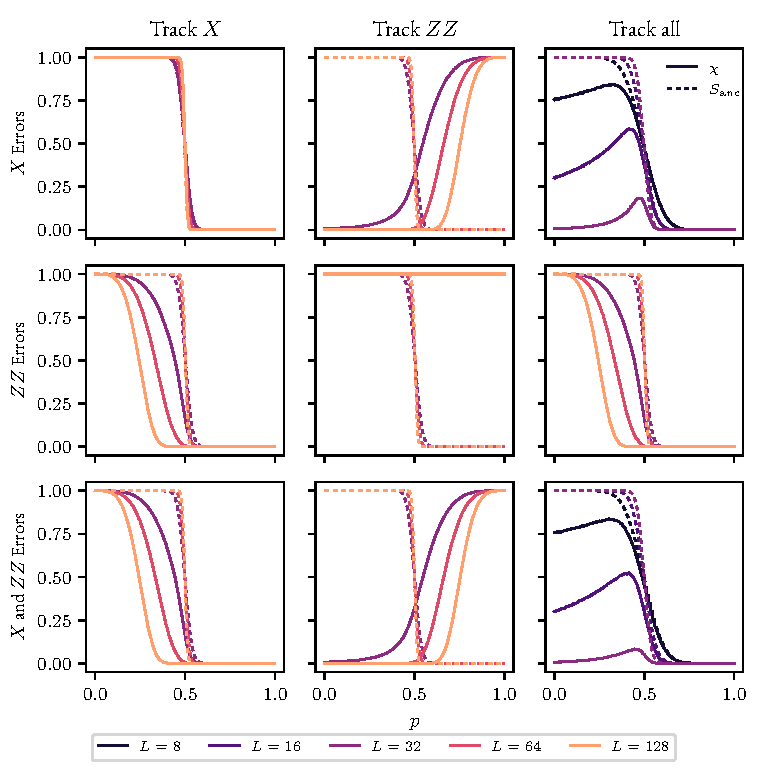
\includegraphics{errors-vs-tracked.pdf}
  \caption{Which measurement outcomes have been tracked and used to compute the
  linear cross entropy, vs the type of errors simulated.}
  \label{fig:err-vs-tra}
\end{figure}
It didn't seem to do so, so i passed \texttt{[h!]}

\begin{figure}[h]
  \centering
  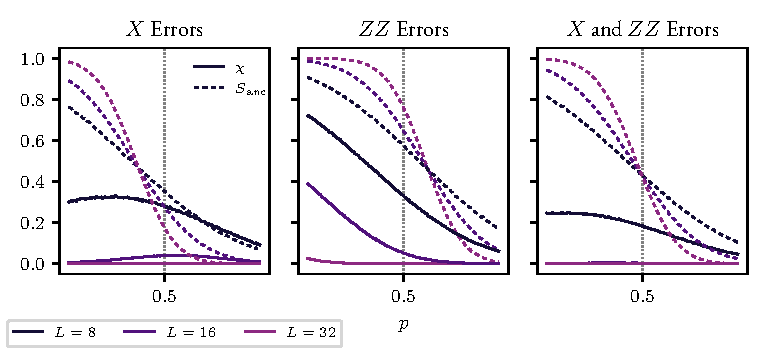
\includegraphics{anc_vs_lxe.pdf}
  \caption{Ancilla entanglement entropy and linear cross entropy for an error
  rate of $q=0.1$ to highlight the behavior of $S_\mathrm{anc}$. The system sizes are chosen smaller compared to
\cref{fig:err-vs-tra} since $\chi$ would be $0$ for larger systems. Note that
this is shown for the region around the critical point $p=.5$ in the ideal
case. This was done to make the shift of $S_\mathrm{anc}$ in $p$ more
noticeable without having the cross entropy be $0$ for ridiculously small
system sizes. Grey vertical dots indicate the critical point in the ideal case
of no errors.}
  \label{fig:large-q-anc-vs-lxe}
\end{figure}
